%%%%%%%%%%%%%%%%%%%%%%%%%%%%%%%%%%%%%%%%%
% Beamer Presentation
% LaTeX Template
% Version 1.0 (10/11/12)
%
% This template has been downloaded from:
% http://www.LaTeXTemplates.com
%
% License:
% CC BY-NC-SA 3.0 (http://creativecommons.org/licenses/by-nc-sa/3.0/)
%
%%%%%%%%%%%%%%%%%%%%%%%%%%%%%%%%%%%%%%%%%

%----------------------------------------------------------------------------------------
%	PACKAGES AND THEMES
%----------------------------------------------------------------------------------------

%\documentclass[UTF8,aspectratio=169,14pt]{ctexbeamer}
\documentclass[UTF8,aspectratio=169]{ctexbeamer}
\usepackage{hyperref}
\hypersetup{
	colorlinks=true,
	linkcolor=red,
	anchorcolor=blue,
	citecolor=green
}

\mode<presentation> {
	
	% The Beamer class comes with a number of default slide themes
	% which change the colors and layouts of slides. Below this is a list
	% of all the themes, uncomment each in turn to see what they look like.
	
	%\usetheme{default}
	%\usetheme{AnnArbor}
	%\usetheme{Antibes}
	%\usetheme{Bergen}
	%\usetheme{Berkeley}
	%\usetheme{Berlin}
	%\usetheme{Boadilla}
	%\usetheme{CambridgeUS}
	%\usetheme{Copenhagen}
	%\usetheme{Darmstadt}
	%\usetheme{Dresden}
	%\usetheme{Frankfurt}
	%\usetheme{Goettingen}
	%\usetheme{Hannover}
	%\usetheme{Ilmenau}
	%\usetheme{JuanLesPins}
	%\usetheme{Luebeck}
	\usetheme{Madrid}
	%\usetheme{Malmoe}
	%\usetheme{Marburg}
	%\usetheme{Montpellier}
	%\usetheme{PaloAlto}
	%\usetheme{Pittsburgh}
	%\usetheme{Rochester}
	%\usetheme{Singapore}
	%\usetheme{Szeged}
	%\usetheme{Warsaw}
	
	% As well as themes, the Beamer class has a number of color themes
	% for any slide theme. Uncomment each of these in turn to see how it
	% changes the colors of your current slide theme.
	
	%\usecolortheme{albatross}
	%\usecolortheme{beaver}
	%\usecolortheme{beetle}
	%\usecolortheme{crane}
	%\usecolortheme{dolphin}
	%\usecolortheme{dove}
	%\usecolortheme{fly}
	%\usecolortheme{lily}
	%\usecolortheme{orchid}
	%\usecolortheme{rose}
	%\usecolortheme{seagull}
	%\usecolortheme{seahorse}
	%\usecolortheme{whale}
	%\usecolortheme{wolverine}
	
	%\setbeamertemplate{footline} % To remove the footer line in all slides uncomment this line
	%\setbeamertemplate{footline}[page number] % To replace the footer line in all slides with a simple slide count uncomment this line
	
	%\setbeamertemplate{navigation symbols}{} % To remove the navigation symbols from the bottom of all slides uncomment this line
}

\usepackage{graphicx} % Allows including images
\graphicspath{{./figs/}}
\usepackage{booktabs} % Allows the use of \toprule, \midrule and \bottomrule in tables
\usepackage{longtable}
\usepackage{listings}
\usepackage{xcolor}
\lstset{numbers=left, %设置行号位置
	numberstyle=\tiny, %设置行号大小
	keywordstyle=\color{blue}, %设置关键字颜色
	commentstyle=\color[cmyk]{1,0,1,0}, %设置注释颜色
	frame=single, %设置边框格式
	escapeinside=``, %逃逸字符(1左面的键),用于显示中文
	%breaklines, %自动折行
	extendedchars=false, %解决代码跨页时,章节标题,页眉等汉字不显示的问题
	xleftmargin=2em,xrightmargin=2em, aboveskip=1em, %设置边距
	tabsize=4, %设置tab空格数
	showspaces=false %不显示空格
}
% Fonts
% \usepackage{libertine}
% \setmonofont{Courier}
\setCJKsansfont[ItalicFont=Noto Serif CJK SC Black, BoldFont=Noto Sans CJK SC Black]{Noto Sans CJK SC}
\setmainfont[Ligatures={Common,TeX}]{Linux  Libertine O}
\setmonofont[SmallCapsFont={Latin Modern Mono Caps}]{Latin Modern Mono Light}
\setsansfont{Linux Biolinum O}

\logo{
\includegraphics[width=0.55cm,height=0.55cm]{../../thcs-logo.png}}

%----------------------------------------------------------------------------------------
%	TITLE PAGE
%----------------------------------------------------------------------------------------

\title[第1讲]{第1讲 :Advanced OS Overview} % The short title appears at the bottom of every slide, the full title is only on the title page
\subtitle{第四节:Tendency of OS -- Performance}
\author{陈渝} % Your name
\institute[清华大学] % Your institution as it will appear on the bottom of every slide, may be shorthand to save space
{
	清华大学计算机系 \\ % Your institution for the title page
	\medskip
	\textit{yuchen@tsinghua.edu.cn} % Your email address
}
\date{\today} % Date, can be changed to a custom date


\begin{document}

\begin{frame}
\titlepage % Print the title page as the first slide
\end{frame}

%\begin{frame}
%\frametitle{提纲} % Table of contents slide, comment this block out to remove it
%\tableofcontents % Throughout your presentation, if you choose to use \section{} and \subsection{} commands, these will automatically be printed on this slide as an overview of your presentation
%\end{frame}
%
%%----------------------------------------------------------------------------------------
%%	PRESENTATION SLIDES
%%----------------------------------------------------------------------------------------
%
%%------------------------------------------------
%\section{第一节:课程概述} % Sections can be created in order to organize your presentation into discrete blocks, all sections and subsections are automatically printed in the table of contents as an overview of the talk
%%------------------------------------------------
%-------------------------------------------------
\begin{frame}
	\frametitle{Tendency}

	\begin{itemize}\huge
	\item \textbf{Performance}
	\item Reliability
	\item Correctness
	
\end{itemize}
\end{frame}


%----------------------------------------------
\begin{frame}[plain]	
	\frametitle{Multi-Core Challenges}
	
	\begin{itemize}\Large
		\item Today's Commodity Multi-Cores
		\item More cores can be integrated
		\begin{itemize}\Large
			\item E.g. Intel's 48-core chip \& AMD's 64-core chip
			\item More cores can be integrated, 1000+ cores (<10years)

	\centering
	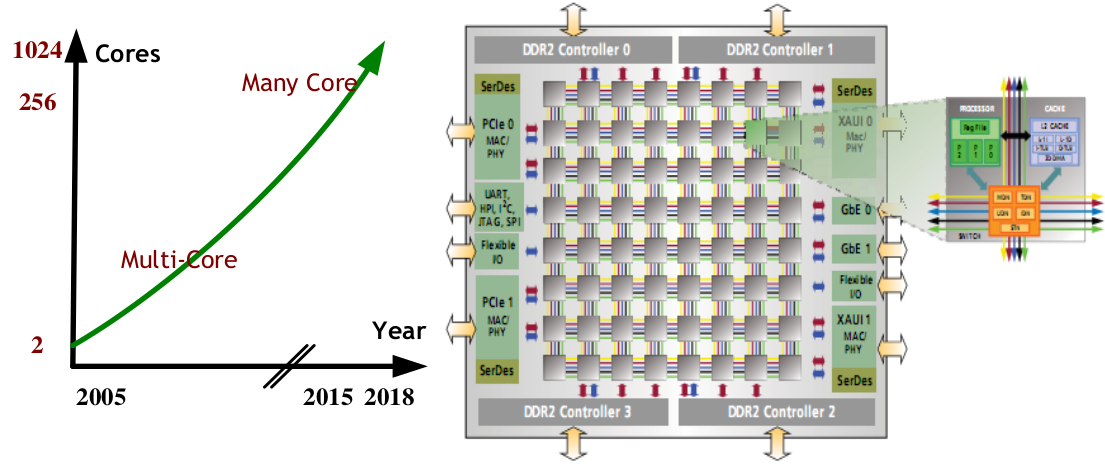
\includegraphics[width=0.6\textwidth]{multicore}
			
		\end{itemize}\pause
	\item However, can operating systems and applications use
	these cores effectively?
	\end{itemize}

	
\end{frame}


%----------------------------------------------
\begin{frame}
	\frametitle{ }
	\begin{columns}
		\begin{column}{.5\textwidth}
			
		\begin{itemize}\LARGE
			\item Linux
			\item Solaris
			\item FreeBSD
			\item Windows
			\item VxWorks
			
		\end{itemize}
			
		\end{column}
		
		\begin{column}{.5\textwidth}
			
			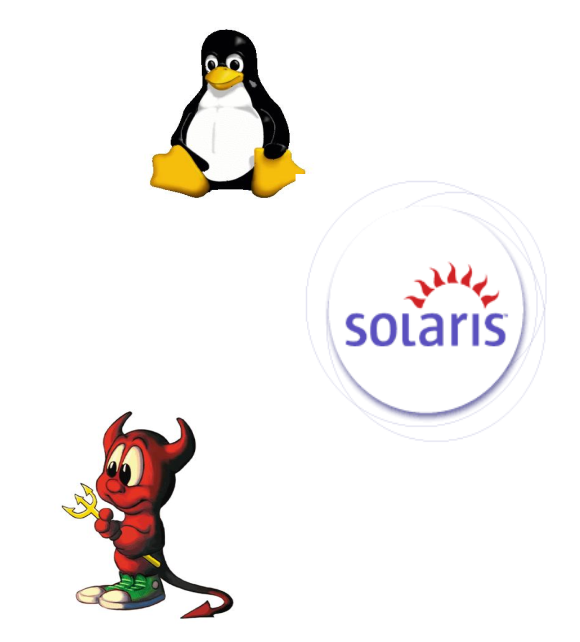
\includegraphics[width=0.8\textwidth]{linux-solaris-freebsd}
			
		\end{column}
	\end{columns}
\end{frame}

%----------------------------------------------
\begin{frame}
	\frametitle{ }
	\begin{columns}
		\begin{column}{.3\textwidth}
			
			\begin{itemize}\LARGE
				\item Linux
				\item Solaris
				\item FreeBSD
				\item Windows
				\item VxWorks
				
			\end{itemize}
			
		\end{column}
		
		\begin{column}{0.7\textwidth}
			
			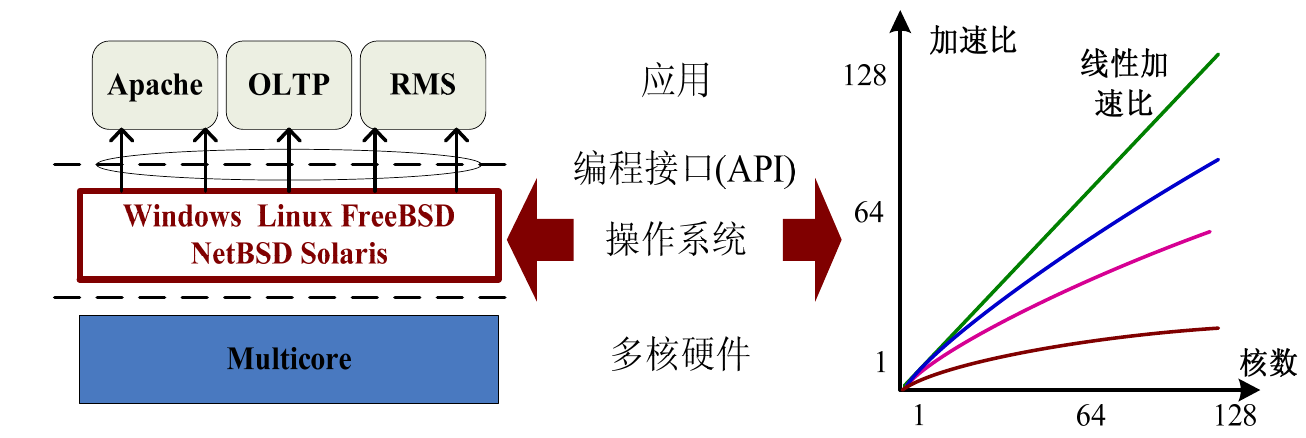
\includegraphics[width=1.0\textwidth]{os-multicore}
			
		\end{column}
	\end{columns}
\end{frame}

%----------------------------------------------
\begin{frame}
	\frametitle{ }
	\begin{columns}[t]
		\begin{column}{.3\textwidth}
			\begin{itemize}\LARGE
				\item Linux
				\item Solaris
				\item FreeBSD
				\item Windows
				\item VxWorks
				
			\end{itemize}
			
		\end{column}
		
		\begin{column}{0.7\textwidth}
			
			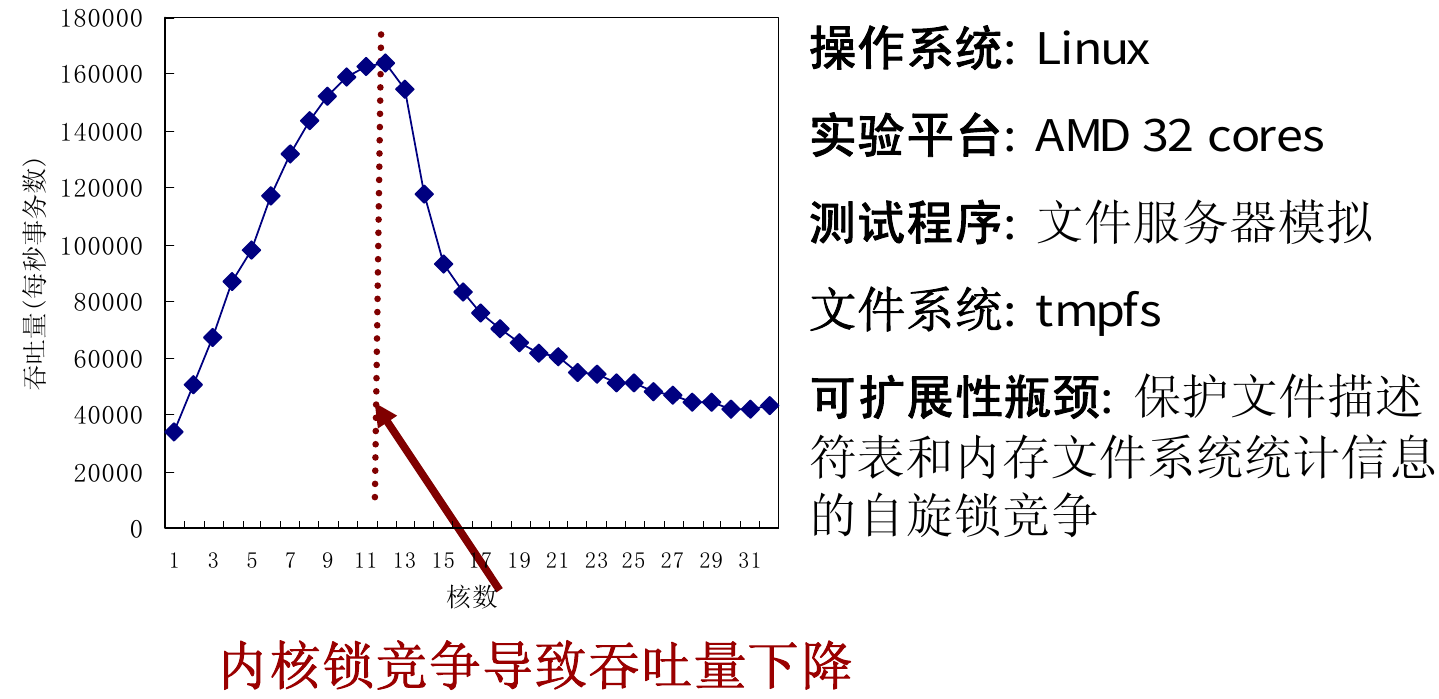
\includegraphics[width=1.0\textwidth]{lock-multicore}
			
		\end{column}
	\end{columns}
\end{frame}

%----------------------------------------------
\begin{frame}[plain]	
	\frametitle{Some Conclusions}
	
	\begin{itemize}\Large
		\item No system scales clearly better than another in
		all aspects for micro-benchmark test
		\item Linux and Solaris are competitive in application
		benchmark test, FreeBSD loses both in
		performance and scalability
		\item Kernel synchronizations protecting the shared
		data structure are the main bottlenecks on multi-
		core platform
		
	\end{itemize}	
	
\end{frame}
%----------------------------------------------
%----------------------------------------------
\end{document}